\documentclass[tikz,border=6pt]{standalone}
\usepackage{xcolor}
\begin{document}
% Canonical ch-diagram for 10_2^0,-2
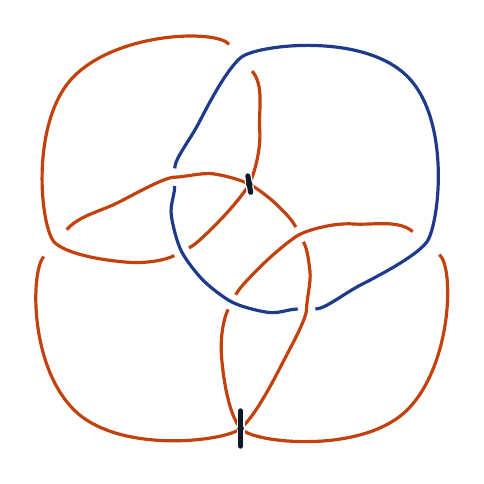
\begin{tikzpicture}[line join=round]
  \definecolor{skcomp0}{RGB}{30,58,138}
  \definecolor{skcomp1}{RGB}{194,65,12}
  \definecolor{skmark}{RGB}{15,23,42}
  \draw[skcomp0, line width=1.15pt, line cap=butt] (-0.8529,0.7094) .. controls (-0.8529,0.5903) and (-0.9140,0.4766) .. (-0.8957,0.3354);
  \draw[skcomp0, line width=1.15pt, line cap=butt] (-0.8529,0.9335) .. controls (-0.8529,1.0596) and (-0.6593,1.2894) .. (-0.5377,1.5267);
  \draw[skcomp1, line width=1.15pt, line cap=butt] (-2.2242,0.1542) .. controls (-2.0690,0.3348) and (-1.7956,0.3845) .. (-1.5582,0.5062);
  \draw[skcomp1, line width=1.15pt, line cap=butt] (-0.1619,2.5088) .. controls (-0.3263,2.7000) and (-1.5655,2.6685) .. (-2.1328,2.1013);
  \draw[skcomp1, line width=1.15pt, line cap=butt] (-2.5165,-0.1857) .. controls (-2.6809,-0.3769) and (-2.7000,-1.5655) .. (-2.1328,-2.1328);
  \draw[skcomp1, line width=1.15pt, line cap=butt] (-0.8582,-0.1741) .. controls (-0.9633,-0.2285) and (-1.1914,-0.2761) .. (-1.4463,-0.2587);
  \draw[skcomp1, line width=1.15pt, line cap=butt] (-0.6715,-0.0772) .. controls (-0.5664,-0.0227) and (-0.4136,0.1384) .. (-0.2918,0.2603);
  \draw[skcomp1, line width=1.15pt, line cap=butt] (0.6849,0.1875) .. controls (0.6335,0.2867) and (0.5498,0.3669) .. (0.4584,0.4584);
  \draw[skcomp1, line width=1.15pt, line cap=butt] (0.1304,2.1689) .. controls (0.2869,1.9868) and (0.2098,1.6696) .. (0.2272,1.4148);
  \draw[skcomp1, line width=1.15pt, line cap=butt] (2.5088,-0.1619) .. controls (2.7000,-0.3263) and (2.6685,-1.5655) .. (2.1013,-2.1328);
  \draw[skcomp1, line width=1.15pt, line cap=butt] (-0.1741,-0.8582) .. controls (-0.2285,-0.9633) and (-0.2761,-1.1914) .. (-0.2587,-1.4463);
  \draw[skcomp0, line width=1.15pt, line cap=butt] (0.7094,-0.8529) .. controls (0.5903,-0.8529) and (0.4766,-0.9140) .. (0.3354,-0.8957);
  \draw[skcomp1, line width=1.15pt, line cap=butt] (-0.0772,-0.6715) .. controls (-0.0227,-0.5664) and (0.1384,-0.4136) .. (0.2603,-0.2918);
  \draw[skcomp1, line width=1.15pt, line cap=butt] (0.7818,0.0007) .. controls (0.8349,-0.1016) and (0.8458,-0.2258) .. (0.8642,-0.3669);
  \draw[skcomp1, line width=1.15pt, line cap=butt] (2.1689,0.1304) .. controls (1.9868,0.2869) and (1.6696,0.2098) .. (1.4148,0.2272);
  \draw[skcomp0, line width=1.15pt, line cap=butt] (0.9335,-0.8529) .. controls (1.0596,-0.8529) and (1.2894,-0.6593) .. (1.5267,-0.5377);
  \draw[skcomp0, line width=1.15pt, line cap=round] (-0.7648,-0.1256) .. controls (-0.8179,-0.0233) and (-0.8773,0.1943) .. (-0.8957,0.3354);
  \draw[skcomp1, line width=1.15pt, line cap=round] (-0.8529,0.8214) .. controls (-0.7338,0.8214) and (-0.5081,0.8825) .. (-0.3669,0.8642);
  \draw[skcomp1, line width=1.15pt, line cap=round] (0.0941,0.7334) .. controls (-0.0082,0.7864) and (-0.2258,0.8458) .. (-0.3669,0.8642);
  \draw[skcomp0, line width=1.15pt, line cap=round] (-0.0157,2.3389) .. controls (-0.1963,2.1836) and (-0.4160,1.7641) .. (-0.5377,1.5267);
  \draw[skcomp1, line width=1.15pt, line cap=round] (-0.8529,0.8214) .. controls (-0.9790,0.8214) and (-1.3209,0.6279) .. (-1.5582,0.5062);
  \draw[skcomp1, line width=1.15pt, line cap=round] (-2.3704,-0.0157) .. controls (-2.5615,0.1486) and (-2.7000,1.5340) .. (-2.1328,2.1013);
  \draw[skcomp1, line width=1.15pt, line cap=round] (-0.0157,-2.3704) .. controls (-0.2069,-2.5347) and (-1.5655,-2.7000) .. (-2.1328,-2.1328);
  \draw[skcomp1, line width=1.15pt, line cap=round] (-2.3704,-0.0157) .. controls (-2.1883,-0.1723) and (-1.7011,-0.2413) .. (-1.4463,-0.2587);
  \draw[skcomp0, line width=1.15pt, line cap=round] (-0.7648,-0.1256) .. controls (-0.7134,-0.2248) and (-0.5813,-0.3984) .. (-0.4899,-0.4899);
  \draw[skcomp0, line width=1.15pt, line cap=round] (-0.1256,-0.7648) .. controls (-0.2248,-0.7134) and (-0.3984,-0.5813) .. (-0.4899,-0.4899);
  \draw[skcomp1, line width=1.15pt, line cap=round] (0.0941,0.7334) .. controls (0.0396,0.6283) and (-0.1699,0.3821) .. (-0.2918,0.2603);
  \draw[skcomp1, line width=1.15pt, line cap=round] (0.0941,0.7334) .. controls (0.1934,0.6819) and (0.3669,0.5498) .. (0.4584,0.4584);
  \draw[skcomp1, line width=1.15pt, line cap=round] (0.0941,0.7334) .. controls (0.1486,0.8384) and (0.2446,1.1599) .. (0.2272,1.4148);
  \draw[skcomp0, line width=1.15pt, line cap=round] (-0.0157,2.3389) .. controls (0.1754,2.5033) and (1.5340,2.6685) .. (2.1013,2.1013);
  \draw[skcomp0, line width=1.15pt, line cap=round] (2.3389,-0.0157) .. controls (2.5033,0.1754) and (2.6685,1.5340) .. (2.1013,2.1013);
  \draw[skcomp1, line width=1.15pt, line cap=round] (-0.0157,-2.3704) .. controls (0.1486,-2.5615) and (1.5340,-2.7000) .. (2.1013,-2.1328);
  \draw[skcomp1, line width=1.15pt, line cap=round] (-0.0157,-2.3704) .. controls (0.1648,-2.2151) and (0.3845,-1.7956) .. (0.5062,-1.5582);
  \draw[skcomp1, line width=1.15pt, line cap=round] (0.8214,-0.8529) .. controls (0.8214,-0.9790) and (0.6279,-1.3209) .. (0.5062,-1.5582);
  \draw[skcomp1, line width=1.15pt, line cap=round] (-0.0157,-2.3704) .. controls (-0.1723,-2.1883) and (-0.2413,-1.7011) .. (-0.2587,-1.4463);
  \draw[skcomp0, line width=1.15pt, line cap=round] (-0.1256,-0.7648) .. controls (-0.0233,-0.8179) and (0.1943,-0.8773) .. (0.3354,-0.8957);
  \draw[skcomp1, line width=1.15pt, line cap=round] (0.7334,0.0941) .. controls (0.6283,0.0396) and (0.3821,-0.1699) .. (0.2603,-0.2918);
  \draw[skcomp1, line width=1.15pt, line cap=round] (0.8214,-0.8529) .. controls (0.8214,-0.7338) and (0.8825,-0.5081) .. (0.8642,-0.3669);
  \draw[skcomp1, line width=1.15pt, line cap=round] (0.7334,0.0941) .. controls (0.8384,0.1486) and (1.1599,0.2446) .. (1.4148,0.2272);
  \draw[skcomp0, line width=1.15pt, line cap=round] (2.3389,-0.0157) .. controls (2.1836,-0.1963) and (1.7641,-0.4160) .. (1.5267,-0.5377);
  \draw[white, line width=2.8pt, line cap=round] (0.0766,0.8371) -- (0.1116,0.6296);
  \draw[skmark, line width=1.85pt, line cap=round] (0.0766,0.8371) -- (0.1116,0.6296);
  \fill[skmark] (0.0941,0.7334) circle (1.2pt);
  \draw[white, line width=2.8pt, line cap=round] (-0.0157,-2.1462) -- (-0.0157,-2.5945);
  \draw[skmark, line width=1.85pt, line cap=round] (-0.0157,-2.1462) -- (-0.0157,-2.5945);
  \fill[skmark] (-0.0157,-2.3704) circle (1.2pt);
\end{tikzpicture}
\end{document}
